\section{Optimizations}
\label{sec:optimizations}

% TODO: Much of the feedback from the OOPSLA reviewers complained in the inadequate
%   context for many of these features, as well as the lack of detail of design
%   choices made in them. Since we are even more space-constrained than the last time,
%   we should prioritize carefully which ones we will discuss and go into detail on
%   the design choices made and differences from other frameworks.}

A high-level IR by itself does not provide a path to high-performance code.
Obtaining high-performance models requires domain-specific
  optimizations tailored to deep learning.
In this section, we showcase the use of the \relay compiler framework
  to write general, domain-specific, and target-specific optimizations,
  enabling generation of high-performance code.

\subsection{Operator Fusion}
\label{sec:fusion}

Operator fusion is an indispensable optimization in deep learning compilers.
Fusion enables better sharing of computation, removal of
  intermediate allocations, and facilitates further optimization by
  combining loop nests.
Fusion is known to be the most critical optimization in machine
  learning compilers, but existing fusion techniques
  are closed (working over a fixed set of ops)
  and target-dependent.
Traditional operator fusion algorithms resemble instruction
  selection:
A sequence of operators eligible
  for fusion is first identified and then replaced with a corresponding
  handwritten fused implementation, usually from a vendor-provided library.
For example, if a fused implementation for a GPU operator does not exist in CuDNN,
  it will remain unfused.
More advanced strategies, implemented in XLA, detect a
  closed set of statically shaped operators for fusion and
  generate code for CPU/GPU.

\relay's fusion algorithm addresses weaknesses of previous approaches by representing
  \textit{all} operators in a secondary IR.
\relay operators are backed by a TVM compute expression that
  describes operations in a high-level DSL that resembles Einstein notation
  but omits low-level scheduling details.
TVM's separation of compute and scheduling provides many favorable qualities
  for \relay's fusion algorithm.
It enables producing shape-specialized fused operators for an open set of operators,
  fusing arbitrary-length chains of operators (not just pairwise combinations),
  and handling operators with multiple outputs and nonlinear consumer-producer patterns.
TVM is also able to reschedule after fusion and perform further optimization via auto-tuning.
\relay performs fusion in two steps, detailed below.

\subsection*{Extraction}

First, \relay identifies subexpressions containing
  fusion-eligible and factors them into local functions that
  are marked as primitive.
Primitive functions can later be lowered to platform-specific
  code.
Fusion-eligible subexpressions are identified by constructing a
  directed acyclic graph (DAG) representing data flow between operators.
As the dataflow DAG is acyclic, it allows for the simple construction
  of a post-dominator tree.
Subexpressions are grouped into equivalence classes
  determined by their immediate post-dominator.
The use of the post-dominator tree enables fusion
  between non-linear producer-consumer relationships;
  for example, \relay can fuse diamond-shaped data-flow relations,
  where an input is used by multiple parallel operator chains
  that are combined again by a later operator.
Finally, \relay constructs an expression from each equivalence class,
  collects the expressions' free variables,
  constructs a function with the expression as the body and the free variables
  as parameters,
  and marks it as primitive.

\subsection*{Lowering}

In a second step, the \relay compiler converts the generated primitive
  function into platform and shape specific code.
For each operator, \relay collects the high-level \tvm expression that represents it,
  then combines them into an aggregate expression that represents the fused operation.
Generating code using \tvm also requires producing a schedule.
It is possible to use \tvm's default schedule to generate code for a single operation,
  but the default schedule does not support fusion.
In order to generate code for the combined expression, we must generate a
  master schedule based on the set of operations being fused.
The fusion algorithm analyzes the expressions to select a master
  schedule, the master schedule will perform the appropriate scheduling
  actions to generate fused code, such as inlining loops, or reorganizing
  computation.
By combining the master schedule with the fused computation,
  \relay is able to produce an optimized version of the operator
  for any platform supported by TVM.
For example, a related project by one of the co-authors implemented
  a RISC-V backend which immediately obtained full operator fusion
  with no new code.
Due to the \relay compiler's integration with AutoTVM, we can further
  optimize fused operations by performing auto-tuning on the master
  schedule template to obtain the best performance.

\subsection{Quantization Framework}
\label{sec:quant}

\begin{figure*}[htbp!]
  \centering
  % TODO: These graphs seem a little small.  Is there any more space hacking we can do?
  \includegraphics[scale=0.53]{fig/eval/graph/quant_comp/raspberry_pi_quantization.png}
  \hspace{-0.075in}
  \includegraphics[scale=0.53]{fig/eval/graph/quant_comp/rk3399_quantization.png}
  % TODO: Use real numbers for this.
  \includegraphics[scale=0.53]{fig/eval/graph/fpga_comp/fpga_eval.png}
  \caption{\textmd{
    \textit{(left)} Inference time of vision DNNs on low-power platforms using
      different data types.
    \relay allows us to reduce inference time on power-constrained devices by
      easily substituting \texttt{float32} multiplications with \texttt{int8}
      multiplications and \texttt{int16} or \texttt{int32} accumulations (denoted
      as \texttt{int8}/\texttt{int16} and \texttt{int8}/\texttt{int32}, respectively).
    We used 1000 trials for each model.
    \textit{(right)}
    Batch-size-normalized inference time of vision DNNs and a TreeLSTM running on two DNN accelerator variants implemented on an edge FPGA.
    One accelerator performs single-batch inference, while the other implements multi-batch inference.
    % Multi-batch inference provides tangible throughput improvements on TreeLSTM due to the memory bandwidth constrained nature of the workload.
    The two hardware designs have the same number of compute units that are arranged differently to take advantage of different types of tensor computation.
    \relay applies a multitude of graph-level transformations required to run different workloads onto these DNN hardware designs.
    We used 12 trials for each model.
  }}
  \label{fig:portability-eval}
\end{figure*}

Deep learning is constrained by memory, compute, and accuracy.
Accuracy is often the only metric optimized by machine learning
  researchers, leading to compute- and memory-hungry models.
The sheer number of parameters and the requisite compute
  makes deploying models to resource-limited devices,
  such as in mobile or IoT, challenging.
Even in non-edge devices, the compute cost of using
  datatypes like FP32 is large and computing with mixed precision
  or reduced precision can aid performance.
Unfortunately, reducing bit-width is not a silver bullet and
  can dramatically harm model accuracy.
The tradeoffs between these quantities has lead to the study of quantized neural networks,
  the process by which NNs are modified to use a smaller precision
  or non-standard datatypes to improve throughput and memory usage.
Quantization is particularly essential for supporting many accelerators due to
  their restricted set of datatypes.

State-of-the-art work on quantization demonstrates a number of tradeoffs
  between different quantization techniques,
  with the best often determined by platform and model type~\citep{krishnamoorthi18}.
Most DL frameworks have chosen a specific set of fixed quantization
  schemes and datatypes due to the effort required to manually implement operators for
  each pairing.

Instead, \relay includes a generic, compiler-based quantization flow that supports a diverse set
  of quantization schemes and can automatically generate code for each one.
\relay provides a general-purpose program-rewriting framework that can be extended
  with per-operator rules, which can annotate inputs and outputs with a datatype
  and precision to quantize to.
Users can overload \relay's existing quantization rewriting rules or add new ones
  to implement different quantization strategies, enabling users to choose between
  signed or unsigned integers or different rounding strategies, such as
  floor, ceiling, or stochastic rounding.

Figure \ref{fig:quant_flow} illustrates the rewriting process.
Furthermore quantization is expanded to standard
  \relay operators, which perform the scaling.
Due to this choice, \relay can then fuse these elementwise operations
  into the original operator, resulting in a brand-new quantized operation.
Finally, \relay can subsequently apply further optimizations like
  layout transformation, accelerator-specific packing, or
  auto-tuning to further improve performance or portability.
This enables the generation of customized quantized operators
  for user-provided schemes and operators,
  not limiting users to a single scheme.

\begin{figure}[h]
  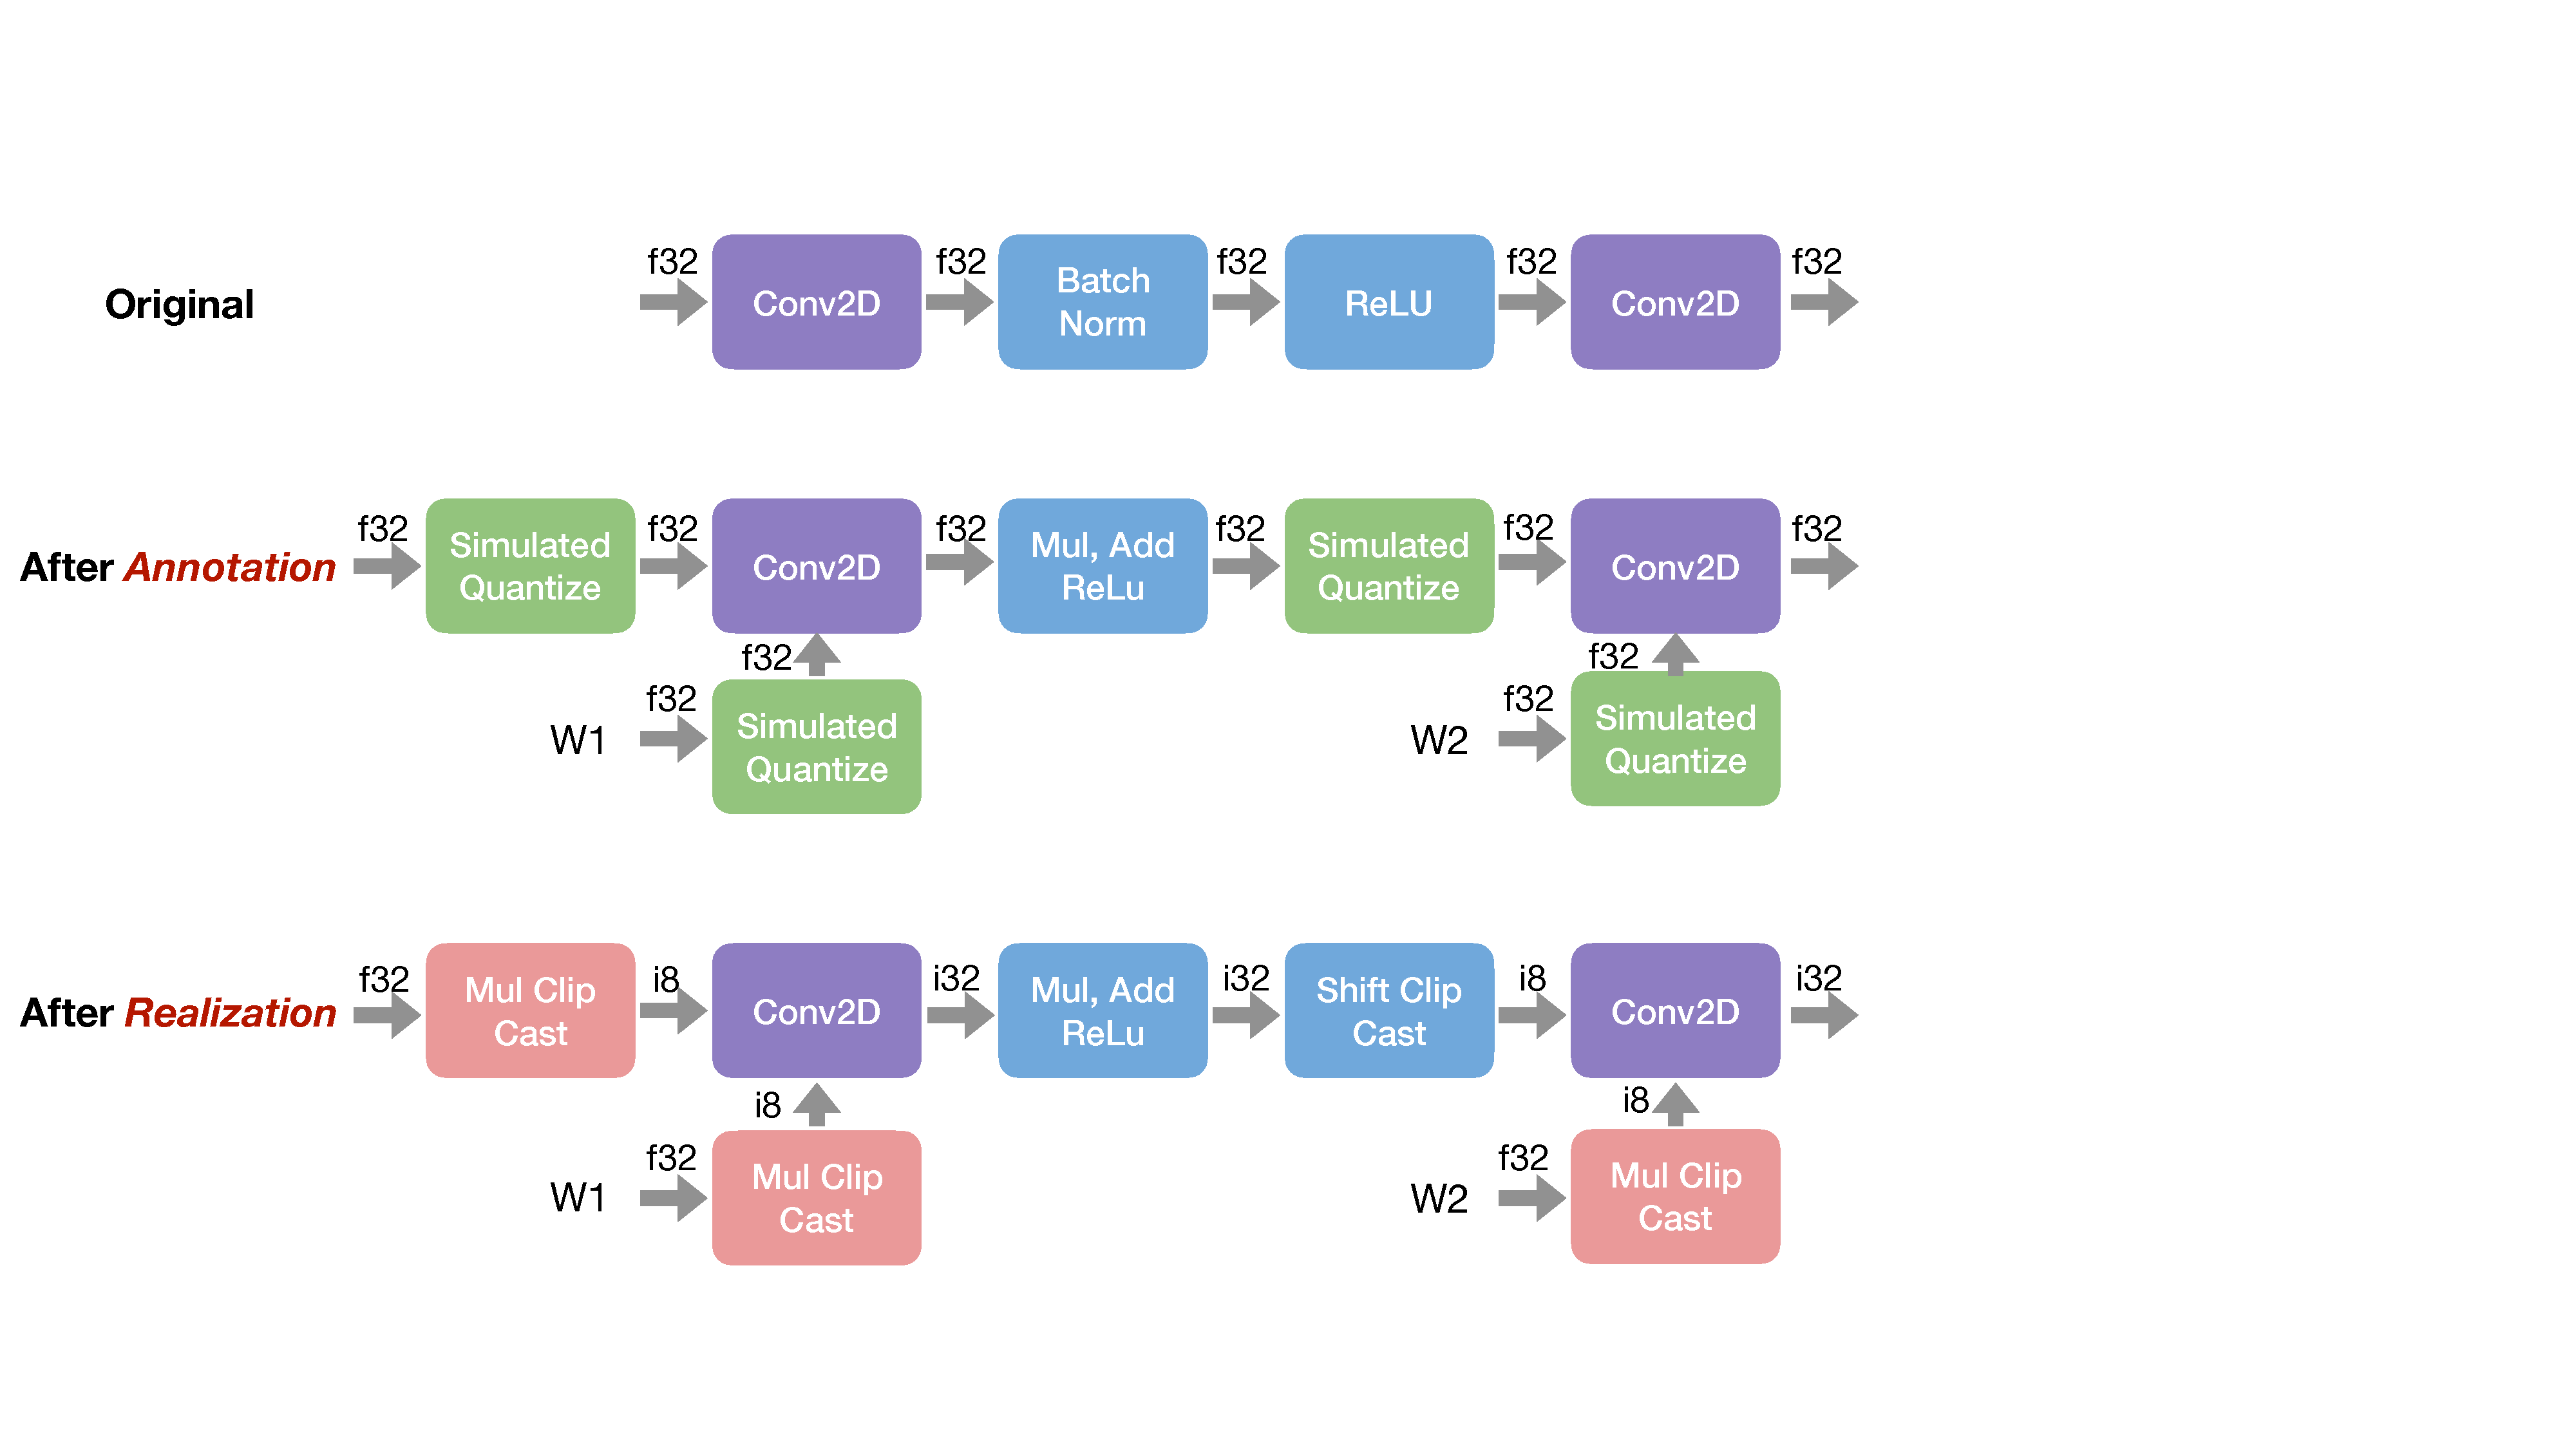
\includegraphics[height=5cm]{fig/quantization/quant_pdf.pdf}
  \caption{\textmd{The top graph represents the dataflow graph of operators after annotation,
  and the bottom graph represents the result of quantization.}}
  \label{fig:quant_flow}
\end{figure}

We will now detail the three steps of the generic quantization flow:
  annotation, calibration, and realization.

\subsection*{Annotate}

Annotation rewrites the program to insert simulated quantization operations
  according to annotation rule for each operator.
Each input or output to be quantized is passed to \texttt{sim$Q$},
  an operator that simulates the effect of quantization (for example, from a 32-bit
  floating point value to an 8-bit integer value).
\texttt{sim$Q$} has a set of parameters that must then be calibrated in order to
  correctly quantize the graph, namely the bits, the scale, and the range.
\texttt{sim$Q$} simulates quantization on
  the unquantized type; that is, it performs computation on the unquantized type
  and then scales it to the target type.
By computing on the unquantized type, \relay can later calibrate the parameters to
  \texttt{sim$Q$} a necessary step to preserve accuracy of the model.
\[
  \texttt{sim$Q$}\left(x, \beta, \sigma, \rho\right) = \dfrac{\texttt{clip}\left(\texttt{round}\left(x / \rho \cdot 2^{\beta - \sigma}\right)\right) \cdot \rho}{2^{\beta - \sigma}}
\]
\subsection*{Calibrate}
As seen above \texttt{sim$Q$} has an input $x$, as well as a number of parameters
  $\beta$, $\sigma$, and $\rho$.
\texttt{sim$Q$}'s parameters control the mapping between the quantized and unquantized type
  and must be calibrated, without calibration the model can be wildly inaccurate.
We must perform an auxiliary optimization task to find the appropriate
  setting for these parameters.
The \relay compiler supports a variety of strategies for setting these
  parameters.
The first strategy implemented is a hyper parameter sweep of a
  single global scale until such a scale is found that does not result
  in overflow.
Another approach is a vision specific scheme which uses
  a per-channel scale, and optimizes the scales using a
  simple mean-squared error loss.
Finally an approach adopted from MxNet uses a
  KL-divergence based loss to optimize the
  quantization scales.

\subsection*{Realize}

Finally, after the algorithm has set the parameters appropriately,
  it applies realization,
  which transforms the \texttt{sim$Q$} operator into the below
  quantization operator.
\[
  Q\left(x, \rho, \beta, \sigma\right) = \texttt{cast}\left(\texttt{clip}\left(\texttt{round}\left(x / \rho \cdot 2^{\beta-\sigma}\right), \texttt{qtype}\right)\right)
\]
The produced operator performs the necessary scaling
  by realizing the operation as a sequence of finer-grained
  operators such as multiplication and rounding.
The output of original operator is now immediately scaled
  by this new operation.
Due to \relay's handling of fusion
  we are able fuse these scaling operations directly into
  to the original operator, transforming a convolution
  from \verb|fp32| to a type such as \verb|int4|.

\subsection{Partial Evaluator}
\label{sec:partial_eval}
Existing deep learning IRs have relied on
  a mixture of staging and constant evaluation
  in order to optimize user programs.
Partial evaluation is a generalized form of constant
  evaluation that can reduce partially constant
  programs.
A partial evaluator (PE) allows the use of high-level abstractions
  without limiting code that \textit{could} in practice be
  compiled to a particular target.
\relay is the first compiler to apply partial evaluation
  techniques to deep learning, the
  core approach of which is based on \citep{pe_ref}.
Partial evaluation, when composed with other
  optimizations like fusion, yields a variety
  of useful optimizations without requiring
  a separate implementation of each.
For example, the partial evaluator can be used to perform
  loop unrolling, which then enables further fusion,
  without any additional compiler passes.

\relay's partial evaluator works by defining a interpreter
  where the value domain is partially static values.
The partially static domain represents simple values,
  such as constant tensors, as themselves.
The representations
  of aggregate values mirror their structure; for example,
  tuples become a tuple of partially static values.
The partially static domain represents dynamic values,
  which may not be known until execution time,
  alongside the static values traditionally supported by
  constant evaluators.
Our partial evaluator must solve two important problems:
  managing effectful computations and handling references.
In order to handle effects, the evaluator keeps the generated
  program in A-normal form to ensure effects are properly ordered
  and restrict duplication of effectful computations.
The partial evaluator supports references by
  simulating the store at partial evaluation time.
The explicit store is threaded throughout execution
  and provides a flow-sensitive PE.
Finally, the evaluator constructs a new program with
  the static subcomputations evaluated away.
% The reconstructed program contains all original
%   expressions, as well as evaluated expressions,
%   because interleaving dead-code elimination (DCE) is
%   non-trivial.
% Afterwards, we separately apply DCE.
% The partial evaluator has use cases beyond inference
%   optimizations, separately it enabled the design of an automatic
%   differentiation algorithm that makes use of hard to optimize
%   features such as references of closures, as the partial evaluator
%   can remove unneeded abstraction.

\subsection{Accelerator-Specific Optimizations}
\label{sec:accel-opts}

% \todo{We should rename the subsection and emphasize strongly that these optimizations
%   are necessary for deploying to different hardware backends. We need to hammer on the
%   point that they make it possible to target systems with restricted computing models
%   without having to change the input program and (we'd need eval to back it up) with
%   good performance.}

This subsection focuses on a subset of optimizations necessary to
  compile \relay to deep learning hardware accelerators.
Although DL accelerators form a diverse family of designs,
  one property they have in common is a restricted computing model.
This means that some individual accelerators
  may not be able to solely execute many \relay programs.
For example, many accelerators cannot execute unbounded loops,
  requiring some computation to be scheduled on a host device
  like the CPU.

\textit{Axis scale folding} is an optimization that removes scaling
  operations that occur before or after convolution-like operators.
The multiplication by a scalar is moved through a convolution towards
  its constant inputs, such as parameters.
By moving the scaling operation to a constant weight, we are able
  to compute away the scale using the partial evaluator.
This optimization is required for certain accelerators that lack scalar multipliers~\citep{moreau2018vta}.
In order to target these accelerators,
  we must eliminate \textit{all} scalar operations.

\textit{Parallel convolution combination} is a specialized
  optimization that fuses multiple 2D convolutions that share the same input.
The goal of this pass is to produce a larger kernel for the GPU,
  as each kernel launch on the GPU has overhead.
It was designed with the Inception network \citep{inception} in mind, as it
  contains blocks of convolutions that share the same input.
The entire parallel convolution combination pass,
  including documentation and tests,
  required fewer than 350 lines of code and was contributed
  by a non-\relay affiliated undergraduate student
  in their first contribution to our codebase.
